\documentclass[10pt,handout]{beamer}\usepackage[]{graphicx}\usepackage[]{color}
% maxwidth is the original width if it is less than linewidth
% otherwise use linewidth (to make sure the graphics do not exceed the margin)
\makeatletter
\def\maxwidth{ %
  \ifdim\Gin@nat@width>\linewidth
    \linewidth
  \else
    \Gin@nat@width
  \fi
}
\makeatother

\definecolor{fgcolor}{rgb}{0.345, 0.345, 0.345}
\newcommand{\hlnum}[1]{\textcolor[rgb]{0.686,0.059,0.569}{#1}}%
\newcommand{\hlstr}[1]{\textcolor[rgb]{0.192,0.494,0.8}{#1}}%
\newcommand{\hlcom}[1]{\textcolor[rgb]{0.678,0.584,0.686}{\textit{#1}}}%
\newcommand{\hlopt}[1]{\textcolor[rgb]{0,0,0}{#1}}%
\newcommand{\hlstd}[1]{\textcolor[rgb]{0.345,0.345,0.345}{#1}}%
\newcommand{\hlkwa}[1]{\textcolor[rgb]{0.161,0.373,0.58}{\textbf{#1}}}%
\newcommand{\hlkwb}[1]{\textcolor[rgb]{0.69,0.353,0.396}{#1}}%
\newcommand{\hlkwc}[1]{\textcolor[rgb]{0.333,0.667,0.333}{#1}}%
\newcommand{\hlkwd}[1]{\textcolor[rgb]{0.737,0.353,0.396}{\textbf{#1}}}%
\let\hlipl\hlkwb

\usepackage{framed}
\makeatletter
\newenvironment{kframe}{%
 \def\at@end@of@kframe{}%
 \ifinner\ifhmode%
  \def\at@end@of@kframe{\end{minipage}}%
  \begin{minipage}{\columnwidth}%
 \fi\fi%
 \def\FrameCommand##1{\hskip\@totalleftmargin \hskip-\fboxsep
 \colorbox{shadecolor}{##1}\hskip-\fboxsep
     % There is no \\@totalrightmargin, so:
     \hskip-\linewidth \hskip-\@totalleftmargin \hskip\columnwidth}%
 \MakeFramed {\advance\hsize-\width
   \@totalleftmargin\z@ \linewidth\hsize
   \@setminipage}}%
 {\par\unskip\endMakeFramed%
 \at@end@of@kframe}
\makeatother

\definecolor{shadecolor}{rgb}{.97, .97, .97}
\definecolor{messagecolor}{rgb}{0, 0, 0}
\definecolor{warningcolor}{rgb}{1, 0, 1}
\definecolor{errorcolor}{rgb}{1, 0, 0}
\newenvironment{knitrout}{}{} % an empty environment to be redefined in TeX

\usepackage{alltt}


%\input{slides_header.tex}
\usepackage{graphicx}
\usepackage{hyperref, url}
\hypersetup{colorlinks,citecolor=myorange,filecolor=red,linkcolor=brown,urlcolor=blue}

\usepackage{longtable,booktabs}
\usepackage{amssymb,amsmath}
\usepackage{animate}
\usepackage{subfig}
\usepackage{tikz}
\usetikzlibrary{shapes.geometric, arrows,shapes.symbols,decorations.pathreplacing}
\tikzstyle{startstop} = [rectangle, rounded corners, minimum width=3cm, minimum height=1cm, draw=black, fill=pinkish,text width=3.5cm]
\tikzstyle{startstop2} = [rectangle, rounded corners, minimum width=3cm, minimum height=1cm, draw=black, fill=background,text width=4.5cm]
\tikzstyle{startstop3} = [rectangle, rounded corners, minimum width=3cm, minimum height=1cm, draw=black, fill=beige,text width=3.0cm]
\tikzstyle{startstop4} = [rectangle, rounded corners, minimum width=3cm, minimum height=1cm, draw=black, fill=pinkish,text width=4.5cm]
\tikzstyle{io} = [trapezium, trapezium left angle=70, trapezium right angle=110, minimum width=2cm, minimum height=1cm, text centered, draw=black, fill=blue!30,text width=1.5cm]
\tikzstyle{process} = [rectangle, minimum width=1cm, minimum height=1cm, text centered, draw=black, fill=orange!30,text width=2cm]
\tikzstyle{decision} = [diamond, minimum width=2cm, minimum height=1cm, text centered, draw=black, fill=green!30]
\tikzstyle{arrow} = [thick,->,>=stealth]
\tikzstyle{both} = [thick,<->,>=stealth, red]


% used for tree of stats tests in 001-introduction
\tikzstyle{startstopstats} = [rectangle, rounded corners, minimum width=2cm, minimum height=.5cm,text centered, draw=black, fill=red!30]
\tikzstyle{iostats} = [trapezium, trapezium left angle=70, trapezium right angle=110, minimum width=2cm, minimum height=.5cm, text centered, draw=black, fill=blue!30]
\tikzstyle{processstats} = [rectangle, minimum width=1.5cm, minimum height=.5cm, text centered, draw=black, fill=orange!30]
\tikzstyle{processbigstats} = [rectangle, minimum width=1.5cm, minimum height=.5cm, text centered, draw=black, fill=orange!30,text width=1.6cm]
\tikzstyle{decisionstats} = [rectangle, minimum width=1cm, minimum height=1cm, text centered, draw=black, fill=green!30,text width=1.6cm]
\tikzstyle{decisionbigstats} = [rectangle, minimum width=1cm, minimum height=1cm, text centered, draw=black, fill=yellow!30,text width=2cm]

\usepackage{pifont}% http://ctan.org/pkg/pifont
\newcommand{\cmark}{\ding{51}}%
\newcommand{\xmark}{\ding{55}}%

\usepackage{ulem} % for strikeout

\usepackage{xcolor}
\usepackage{color, colortbl}
\definecolor{lightgray}{RGB}{200,200,200}
\definecolor{palegray}{RGB}{221,221,221}
\definecolor{myblue}{RGB}{0,89,179}
\definecolor{myorange}{rgb}{0.776,0.357,0.157}
\definecolor{gray}{RGB}{110,110,110}
\definecolor{darkgray}{RGB}{100,100,100}
\definecolor{lightgray}{RGB}{200,200,200}
\definecolor{palegray}{RGB}{221,221,221}
\definecolor{turquoise}{RGB}{81,193,188}
\definecolor{tomato}{RGB}{255,136,136}
\definecolor{mandarina}{RGB}{229,169,25}
\definecolor{foreground}{RGB}{81,141,193}
\definecolor{background}{RGB}{246,244,240}
\definecolor{highlight}{RGB}{229,169,25}
\definecolor{lowlight}{RGB}{200,200,200}
\definecolor{beige}{RGB}{255,255,240}
\definecolor{pinkish}{RGB}{255,223,247}
\definecolor{darktangerine}{rgb}{1.0, 0.66, 0.07}
\definecolor{deepink}{RGB}{255,20,147}
%\usepackage{shadethm}
%\colorlet{shadecolor}{blue!15}
%\colorlet{shadecolor}{palegray}
%\setlength{\shadeboxrule}{.4pt}

%\newshadetheorem{thm}{Theorem}
%\newshadetheorem{defm}{Definition}
%\newshadetheorem{exm}{Exercise}
%\newshadetheorem{remarkm}{Remark}
%\definecolor{shadethmcolor}{HTML}{EDF8FF}
%\definecolor{shadethmcolor}{RGB}{221,221,221}
%\definecolor{shaderulecolor}{HTML}{45CFFF}
%\definecolor{shaderulecolor}{RGB}{0,89,179}
%\setlength{\shadeboxrule}{.4pt}



\usepackage{epsfig}

\newcommand{\code}[1]{\texttt{#1}}
\newcommand{\blue}[1]{\textcolor{blue}{#1}}
\newcommand{\red}[1]{\textcolor{red}{#1}}

\usepackage{comment}

\makeatletter

\def \iqsssectiontitleheader {}

\newcommand{\iqsssectiontitle}[1]{
	\def \iqsssectiontitleheader{#1}
}

\@ifundefined{insertmainframenumber}
{%
	% \insertmainframenumber not defined
	\newcommand{\insertmainframenumber}{\inserttotalframenumber}
}
{%
	% \insertmainframenumber already defined
}%


\AtBeginSection[]{
	\title{\insertsectionhead}
	{
		%\definecolor{white}{RGB}{140,193,250}
		%\definecolor{white}{RGB}{200,200,200}
		%\definecolor{white}{RGB}{242,244,247}
		\definecolor{white}{RGB}{0,89,179}
		%\definecolor{iqss@orange}{rgb}{1,1,1}
		\ifnum \insertmainframenumber > \insertframenumber
		%\setbeamercolor{background canvas}{bg=myblue}
		%\setbeamercolor{normal text}{fg=black,bg=white}
		%\setbeamercolor{frametitle}{fg=red}
		%\setbeamercolor{section in toc}{fg=myblue, bg=white}
		%\setbeamercolor{subsection in toc}{fg=myblue, bg=white}
		\frame{
			\frametitle{\iqsssectiontitleheader}
			\tableofcontents[currentsection]
		}
		\else
		\frame{
			\frametitle{Backup Slides}
			\tableofcontents[sectionstyle=shaded/shaded,subsectionstyle=shaded/shaded/shaded]
		}
		\fi
	}
}
\makeatother
%\graphicspath{{/home/sahir/git_repositories/EPIB607/resources/assets/slides/figure/}}


\usepackage{fontspec}
%\setsansfont{Fira Sans}
%\setmonofont{Fira Mono}
%\setsansfont[ItalicFont={Fira Sans Light Italic},BoldFont={Fira Sans},BoldItalicFont={Fira Sans Italic}]{Fira Sans Light}
%\setmonofont[BoldFont={Fira Mono Medium}]{Fira Mono}

\def\installpath{/usr/local/share/texmf/fonts/opentype/libertinus/}
\setmainfont{LibertinusSerif}[
UprightFont    = *-Regular,
BoldFont       = *-Bold,
ItalicFont     = *-Italic,
BoldItalicFont = *-BoldItalic,
Ligatures      = TeX,
Extension      = .otf,
Path           = \installpath/
]

\setsansfont{LibertinusSerif}[
UprightFont    = *-Regular,
BoldFont       = *-Bold,
ItalicFont     = *-Italic,
BoldItalicFont = *-BoldItalic,
Ligatures      = TeX,
Extension      = .otf,
Path           = \installpath/
]


%\setmonofont{LibertinusSerif}[
%UprightFont    = *-Regular,
%BoldFont       = *-Bold,
%ItalicFont     = *-Italic,
%BoldItalicFont = *-BoldItalic,
%Ligatures      = TeX,
%Extension      = .otf,
%Path           = \installpath/
%]






\newcommand\Wider[2][3em]{%
	\makebox[\linewidth][c]{%
		\begin{minipage}{\dimexpr\textwidth+#1\relax}
			\raggedright#2
		\end{minipage}%
	}%
}


\newcommand {\framedgraphic}[1] {
	\begin{figure}
		\centering
		\includegraphics[width=\textwidth,height=0.9\textheight,keepaspectratio]{#1}
	\end{figure}
}


\newcommand {\framedgraphiccaption}[2] {
	\begin{figure}
		\centering
		\includegraphics[width=\textwidth,height=0.8\textheight,keepaspectratio]{#1}
		\caption{#2}
	\end{figure}
}




\setbeamercolor{itemize item}{fg=myblue}
\setbeamercolor{itemize subitem}{fg=myorange}
%\setbeamertemplate{itemize item}[square]
\setbeamertemplate{itemize item}[circle]
\setbeamertemplate{itemize subitem}[triangle]
\setbeamertemplate{blocks}[rounded][shadow=true]
\setbeamercolor{block body alerted}{bg=alerted text.fg!10}
\setbeamercolor{block title alerted}{bg=alerted text.fg!20}
\setbeamercolor{block body}{bg=structure!10}
\setbeamercolor{block title}{bg=structure!20}
\setbeamercolor{block body example}{bg=green!10}
\setbeamercolor{block title example}{bg=green!20}


\makeatletter
\newenvironment<>{proofs}[1][\proofname]{%
	\par
	\def\insertproofname{#1\@addpunct{.}}%
	\usebeamertemplate{proof begin}#2}
{\usebeamertemplate{proof end}}
\newenvironment<>{proofc}{%
	\setbeamertemplate{proof begin}{\begin{block}{}}
		\par
		\usebeamertemplate{proof begin}}
	{\usebeamertemplate{proof end}}
	\newenvironment<>{proofe}{%
		\par
		\pushQED{\qed}
		\setbeamertemplate{proof begin}{\begin{block}{}}
			\usebeamertemplate{proof begin}}
		{\popQED\usebeamertemplate{proof end}}
\makeatother


\makeatletter
\newenvironment<>{exams}[1][\proofname]{%
	\par
	\def\insertproofname{#1\@addpunct{.}}%
	\usebeamertemplate{example begin}#2}
{\usebeamertemplate{example end}}
\newenvironment<>{examc}{%
	\setbeamertemplate{exam begin}{\begin{block}{}}
		\par
		\usebeamertemplate{exam begin}}
	{\usebeamertemplate{exam end}}
	\newenvironment<>{exame}{%
		\par
		\pushQED{\qed}
		\setbeamertemplate{exam begin}{\begin{block}{}}
			\usebeamertemplate{exam begin}}
		{\popQED\usebeamertemplate{exam end}}
		\makeatother

%\definecolor{mycolor}{HTML}{F7F8E0}
%\declaretheorem[shaded={bgcolor=mandarina}]{theo}
%\declaretheorem[shaded={bgcolor=mycolor}]{propo}
%\declaretheorem[shaded={bgcolor=green!80!black!30}]{remark}

%\setbeamertemplate{navigation symbols}{\usebeamercolor[fg]{title in head/foot}\usebeamerfont{title in head/foot}\insertframenumber}


%\setbeamertemplate{footline}{}

\beamertemplatenavigationsymbolsempty % toggle off if you want navigation symbols at the bottom

\setbeamertemplate{footline}
{ \usebeamercolor[fg]{page number in head/foot}%
	\usebeamerfont{page number in head/foot}%
	\hspace{1em}\insertsectionhead%
	\hfill%
	\insertframenumber\,/\,\hyperlinkappendixstart{\insertmainframenumber}
	\ifnum \thepage = \insertframeendpage{\small .}\else{\phantom{\small .}}\fi
	\hspace{1em}
	\vskip2pt%
}

%\newtheorem{proposition}[theorem]{Proposition}
%\newtheorem{exercise}[theorem]{Exercise}
%\newtheorem{remark}[theorem]{Remark}


\usepackage{amsthm}
\usepackage{thmtools}

\setbeamertemplate{theorems}[ams style] 
%\setbeamertemplate{theorems}[numbered] 
%\setbeamertemplate{corollary}[numbered] 
\newtheorem{proposition}{Proposition}
\newtheorem{exercise}{Exercise}
\newtheorem{remark}{Remark}
\newtheorem{exam}{Example}
%\newtheorem{proof}{Proof}
%\newtheorem{corollaries}[theorem]{Corollary}
\newcommand*{\theorembreak}{\usebeamertemplate{theorem end}\framebreak\usebeamertemplate{theorem begin}}



\setlength{\emergencystretch}{3em} % prevent overfull lines
\providecommand{\tightlist}{%
	\setlength{\itemsep}{0pt}\setlength{\parskip}{0pt}}

\newcommand\AddButton{%
	\setbeamertemplate{background canvas}{%
		\begin{tikzpicture}[remember picture,overlay]
		\node[anchor=west] at ([yshift=5pt,xshift=0.1em]current page.south west)
		{\hyperlink{toc}{\beamergotobutton{back to TOC}}};
		\end{tikzpicture}%
	}%
}


\titlegraphic{\hfill
\includegraphics[height=1cm]{/home/sahir/git_repositories/EPIB607/slides/mcgill_logo.png}}




\graphicspath{{/home/sahir/git_repositories/EPIB607/slides/figure/}}

%\let\oldShaded\Shaded
%\let\endoldShaded\endShaded
%\renewenvironment{Shaded}{\footnotesize\oldShaded}{\endoldShaded}
\IfFileExists{upquote.sty}{\usepackage{upquote}}{}
\begin{document}



%\title{Introduction to Regression Trees}
%\author{Sahir Bhatnagar \inst{1}}
%\author[shortname]{Sahir Rai Bhatnagar, PhD Candidate (Biostatistics) }
%\institute[shortinst]{Department of Epidemiology, Biostatistics and Occupational Health}

\title{001 - Introduction to Inferential Statistics}
\author{EPIB 607 - FALL 2020}
\institute{
	Sahir Rai Bhatnagar\\
	Department of Epidemiology, Biostatistics, and Occupational Health\\
	McGill University\\
	
	\vspace{0.1 in}
	
	\texttt{sahir.bhatnagar@mcgill.ca}\\
	%\texttt{\url{https://sahirbhatnagar.com/EPIB607/}}
}

\date{slides compiled on \today}

\maketitle

\section{Objectives}





\begin{frame}{Objectives for this course}

\begin{enumerate}[<+->]

\item Visualize/Analyze/Interpret data using statistical methods with a computer
\item Gather data into analysis ready format
\item Learn regression
\item Understand the statistical results in a scientific paper
\item Learn the tools for creating reproducible analyses

\end{enumerate}

\end{frame}



\section{Visualize/Analyze/Interpret data using statistical methods with a computer}


\begin{frame}{Data is the new oil\footnote{\tiny\url{https://www.economist.com/briefing/2017/05/06/data-is-giving-rise-to-a-new-economy}}}
	\centering
	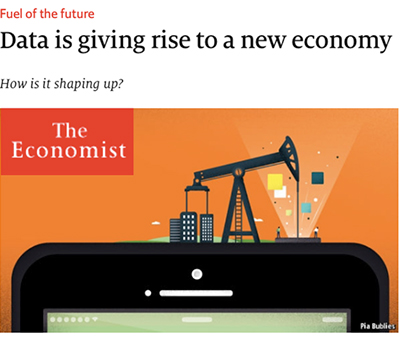
\includegraphics[scale=0.5]{001-oil.jpg}

\end{frame}



\begin{frame}{Danger\footnote{\tiny\url{https://timoelliott.com/blog/2018/03/data-is-the-new-oil-yes-toxic-if-mishandled.html}}}
	\centering
	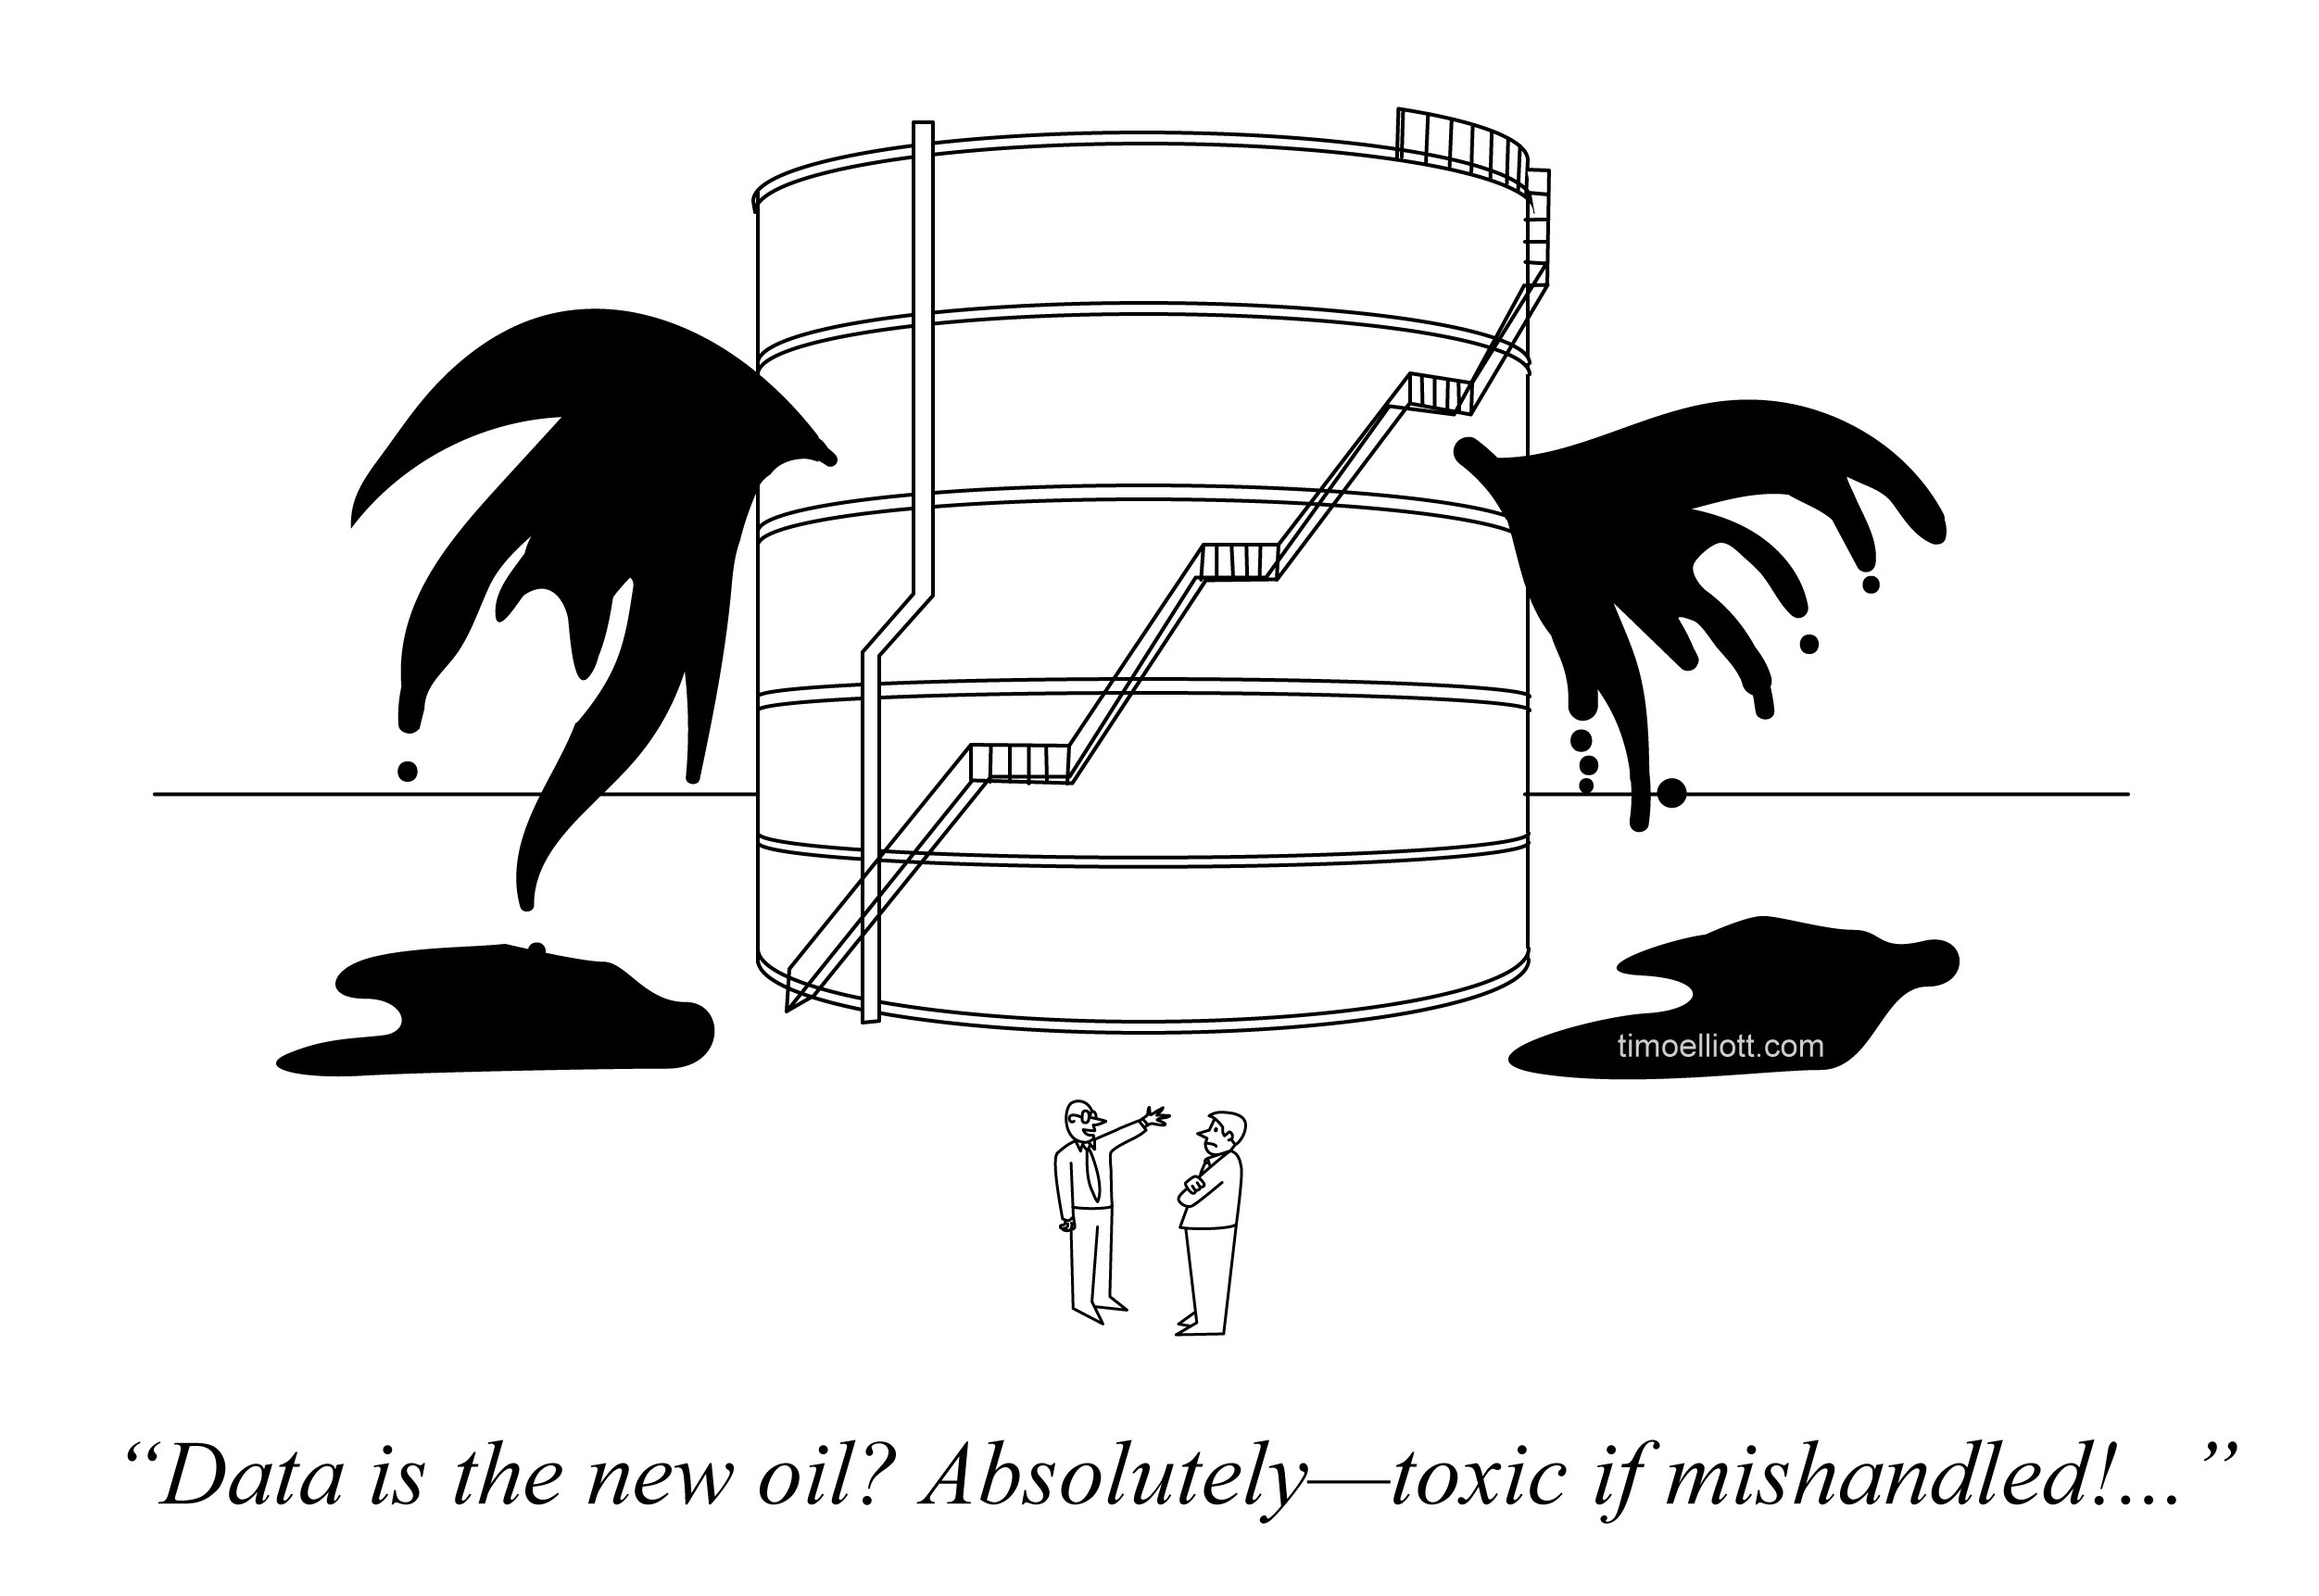
\includegraphics[scale=0.15]{001-toxic.jpg}	
\end{frame}


\begin{frame}{Data science\footnote{\tiny\url{https://hbr.org/2012/10/data-scientist-the-sexiest-job-of-the-21st-century}}}
	\centering
	
\includegraphics[scale=0.35]{001-hbr.png}	
\end{frame}



\begin{frame}{Why \texttt{R} ?}
	\Wider[9em]{
		\begin{figure}
			\begin{minipage}[h]{0.40\linewidth}
				\centering
				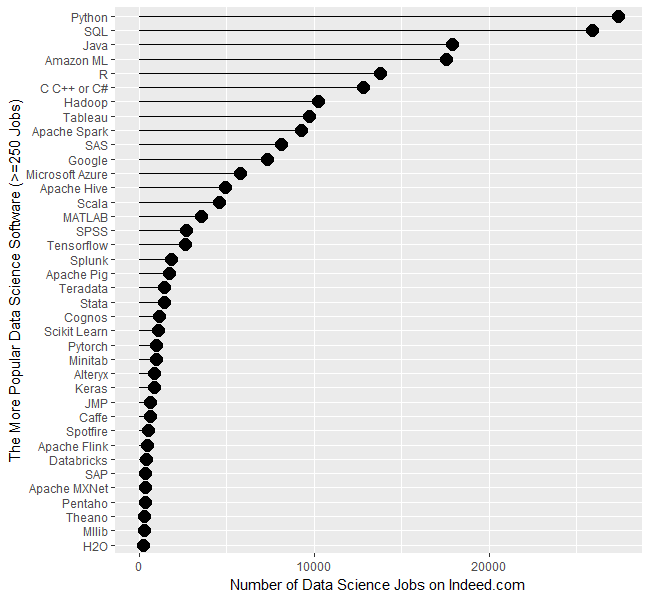
\includegraphics[scale=0.3]{001-rjobs.png}
				\caption{Data as of May 2019 {\tiny \url{http://r4stats.com/articles/popularity/}}}
				\label{fig:a}
			\end{minipage}
			%\hspace{0.5cm}
			\begin{minipage}[h]{0.40\linewidth}
				\centering
				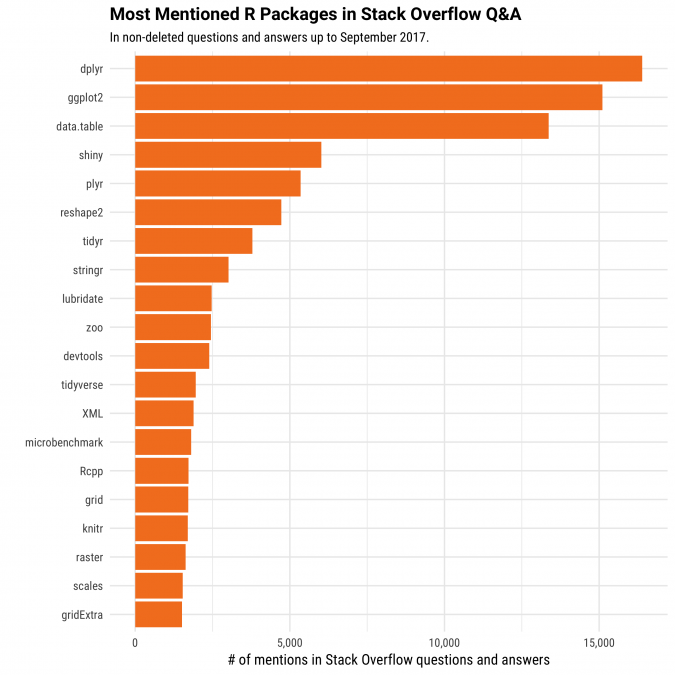
\includegraphics[scale=0.2]{001-dplyr.png}
				\caption{Popular \texttt{R} packages {\tiny \url{https://stackoverflow.blog/2017/10/10/impressive-growth-r/}}}
				\label{fig:b}
			\end{minipage}
		\end{figure}
	}
\end{frame}


\begin{frame}{First day in a statistics course}
\Wider[5em]{
	\centering
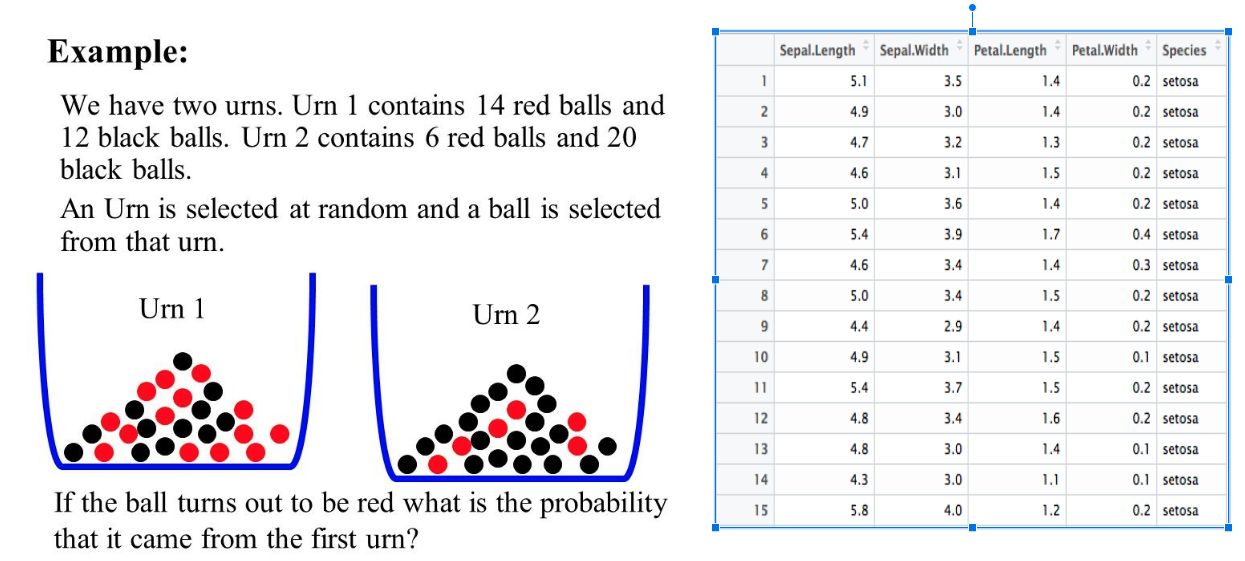
\includegraphics[scale=0.35]{001-firstday.png}
}
\end{frame}


\begin{frame}{Second day in a statistics course}
	\Wider[5em]{
		\centering
		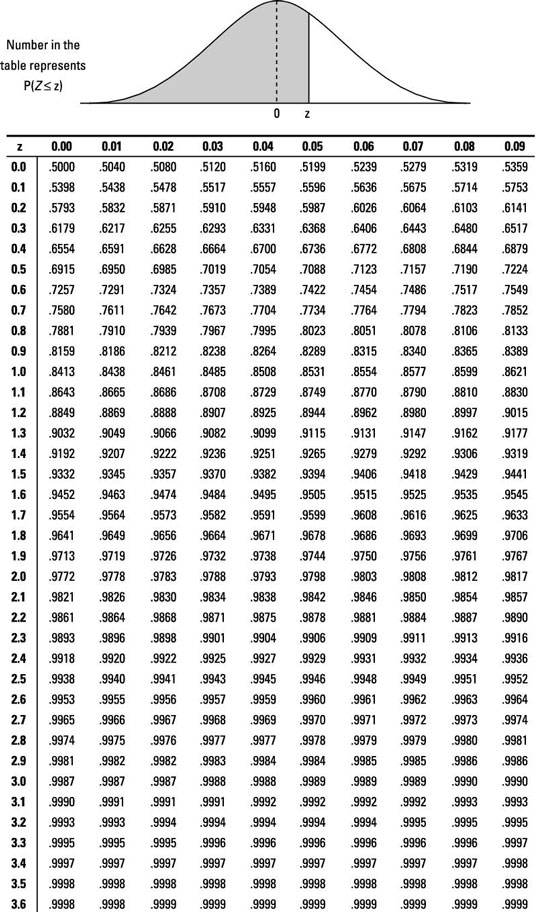
\includegraphics[scale=0.25]{001-ztable.jpg}
	}
\end{frame}

\section{Gather data into analysis ready format}

\begin{frame}{Tidy data}
	
\begin{itemize}
	\setlength\itemsep{.51em}
	\item Each variable forms a column.
	\item Each observation forms a row.
	\item Each type of observational units forms a table
	\item Tidy data is ready for regression routines and plotting
\end{itemize}


\framedgraphic{001-tidy.png}
\end{frame}



\begin{frame}[fragile]{Example: Does a full moon affect behaviour?}
	
	\small
	\begin{itemize}
		\item Many people believe that the moon influences the actions of some individuals. 
		\item A study of dementia patients in nursing homes recorded various types of disruptive behaviors every day for 12 weeks. 
		\item Days were classified as moon days if they were in a 3-day period centered at the day of the full moon. 
		\item For each patient, the average number of disruptive behaviors was computed for moon days and for all otherdays. 
	\end{itemize}
	
\begin{knitrout}\footnotesize
\definecolor{shadecolor}{rgb}{0.969, 0.969, 0.969}\color{fgcolor}
\begin{tabular}{r|r|r}
\hline
patient & moon\_days & other\_days\\
\hline
1 & 3.33 & 0.27\\
\hline
2 & 3.67 & 0.59\\
\hline
3 & 2.67 & 0.32\\
\hline
4 & 3.33 & 0.19\\
\hline
5 & 3.33 & 1.26\\
\hline
6 & 3.67 & 0.11\\
\hline
7 & 4.67 & 0.30\\
\hline
\end{tabular}


\end{knitrout}
	
	
	
\end{frame}


\begin{frame}[fragile]{Is it tidy?}
	
\begin{knitrout}\footnotesize
\definecolor{shadecolor}{rgb}{0.969, 0.969, 0.969}\color{fgcolor}
\begin{tabular}{r|r|r}
\hline
patient & moon\_days & other\_days\\
\hline
1 & 3.33 & 0.27\\
\hline
2 & 3.67 & 0.59\\
\hline
3 & 2.67 & 0.32\\
\hline
\end{tabular}


\end{knitrout}
	
	\pause
	
	\vspace*{0.4cm}
	
	\textcolor{blue}{\textbf{Question: Can I plot the data?}}
	
	\pause
	
\begin{knitrout}\tiny
\definecolor{shadecolor}{rgb}{0.969, 0.969, 0.969}\color{fgcolor}\begin{kframe}
\begin{alltt}
\hlkwd{plot}\hlstd{(df}\hlopt{$}\hlstd{moon_days, df}\hlopt{$}\hlstd{other_days,} \hlkwc{pch} \hlstd{=} \hlnum{19}\hlstd{)}
\hlkwd{abline}\hlstd{(}\hlkwc{a}\hlstd{=}\hlnum{0}\hlstd{,}\hlkwc{b}\hlstd{=}\hlnum{1}\hlstd{)}
\end{alltt}
\end{kframe}

{\centering 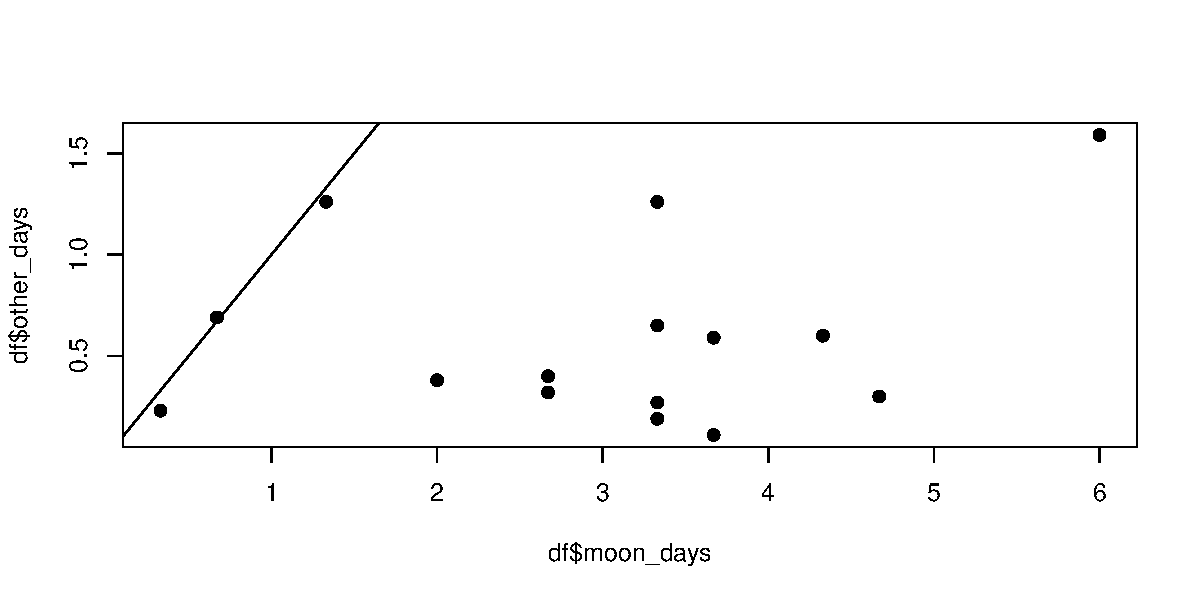
\includegraphics[width=1\linewidth]{figure/unnamed-chunk-3-1} 

}



\end{knitrout}
\end{frame}


\begin{frame}[fragile]{Is it tidy?}
	
\begin{knitrout}\footnotesize
\definecolor{shadecolor}{rgb}{0.969, 0.969, 0.969}\color{fgcolor}
\begin{tabular}{r|r|r}
\hline
patient & moon\_days & other\_days\\
\hline
1 & 3.33 & 0.27\\
\hline
2 & 3.67 & 0.59\\
\hline
3 & 2.67 & 0.32\\
\hline
4 & 3.33 & 0.19\\
\hline
5 & 3.33 & 1.26\\
\hline
\end{tabular}


\end{knitrout}
	
	\pause
	
	\vspace*{0.4cm}
	
	\textcolor{blue}{\textbf{Question: Can I fit a \underline{meaningful} regression model \underline{directly} to the \underline{variables} in the data?}}
	
	\pause
	
\begin{knitrout}\scriptsize
\definecolor{shadecolor}{rgb}{0.969, 0.969, 0.969}\color{fgcolor}\begin{kframe}
\begin{verbatim}
## Call: lm(formula = moon_days ~ other_days, data = df)
## 
## Coefficients:
##             Estimate Std. Error t value Pr(>|t|)
## (Intercept)     2.56       0.66     3.9    0.002
## other_days      0.79       0.91     0.9    0.402
## 
## Residual standard error: 1.5 on 13 degrees of freedom
## Multiple R-squared: 0.055,	Adjusted R-squared: -0.018 
## F-statistic: 0.75 on 1 and 13 DF,  p-value: 0.4
\end{verbatim}
\end{kframe}
\end{knitrout}
\end{frame}






\begin{frame}[fragile]{Is it tidy?}
	
\begin{knitrout}\footnotesize
\definecolor{shadecolor}{rgb}{0.969, 0.969, 0.969}\color{fgcolor}
\begin{tabular}{l|l|r}
\hline
patient & day\_type & mean\_behavior\\
\hline
1 & moon\_days & 3.33\\
\hline
1 & other\_days & 0.27\\
\hline
2 & moon\_days & 3.67\\
\hline
2 & other\_days & 0.59\\
\hline
3 & moon\_days & 2.67\\
\hline
3 & other\_days & 0.32\\
\hline
4 & moon\_days & 3.33\\
\hline
4 & other\_days & 0.19\\
\hline
5 & moon\_days & 3.33\\
\hline
5 & other\_days & 1.26\\
\hline
\end{tabular}


\end{knitrout}
	
	
\end{frame}


\begin{frame}[fragile]{Plotting with tidy data}
	
\begin{knitrout}\tiny
\definecolor{shadecolor}{rgb}{0.969, 0.969, 0.969}\color{fgcolor}\begin{kframe}
\begin{alltt}
\hlkwd{ggplot}\hlstd{(}\hlkwc{data} \hlstd{= df_tidy,} \hlkwc{mapping} \hlstd{=} \hlkwd{aes}\hlstd{(}\hlkwc{x} \hlstd{= day_type,} \hlkwc{y} \hlstd{= mean_behavior,} \hlkwc{group} \hlstd{= patient))} \hlopt{+} \hlkwd{geom_line}\hlstd{()}
\end{alltt}
\end{kframe}
\end{knitrout}
	
\begin{knitrout}\tiny
\definecolor{shadecolor}{rgb}{0.969, 0.969, 0.969}\color{fgcolor}\begin{kframe}


{\ttfamily\noindent\bfseries\color{errorcolor}{Error in loadNamespace(name): there is no package called 'ggpubr'}}\end{kframe}
\end{knitrout}
	
	
\end{frame}



\begin{frame}[fragile]{Regression with tidy data}
	
	
\begin{knitrout}\tiny
\definecolor{shadecolor}{rgb}{0.969, 0.969, 0.969}\color{fgcolor}\begin{kframe}
\begin{alltt}
\hlstd{fit} \hlkwb{<-} \hlstd{lme4}\hlopt{::}\hlkwd{lmer}\hlstd{(mean_behavior} \hlopt{~} \hlstd{day_type} \hlopt{+} \hlstd{(}\hlnum{1}\hlopt{|}\hlstd{patient),} \hlkwc{data} \hlstd{= df_tidy)}
\hlkwd{summary}\hlstd{(fit)}
\end{alltt}
\begin{verbatim}
## Linear mixed model fit by REML ['lmerMod']
## Formula: mean_behavior ~ day_type + (1 | patient)
##    Data: df_tidy
## 
## REML criterion at convergence: 90.3
## 
## Scaled residuals: 
##     Min      1Q  Median      3Q     Max 
## -2.2728 -0.3014 -0.0408  0.4860  2.4482 
## 
## Random effects:
##  Groups   Name        Variance Std.Dev.
##  patient  (Intercept) 0.1559   0.3948  
##  Residual             1.0663   1.0326  
## Number of obs: 30, groups:  patient, 15
## 
## Fixed effects:
##                    Estimate Std. Error t value
## (Intercept)          3.0220     0.2854  10.587
## day_typeother_days  -2.4327     0.3771  -6.452
## 
## Correlation of Fixed Effects:
##             (Intr)
## dy_typthr_d -0.660
\end{verbatim}
\end{kframe}
\end{knitrout}
\end{frame}



\begin{frame}[fragile]{Not tidy vs. tidy data}
	
	
	%\Wider[4em]{
	%\centering
	
	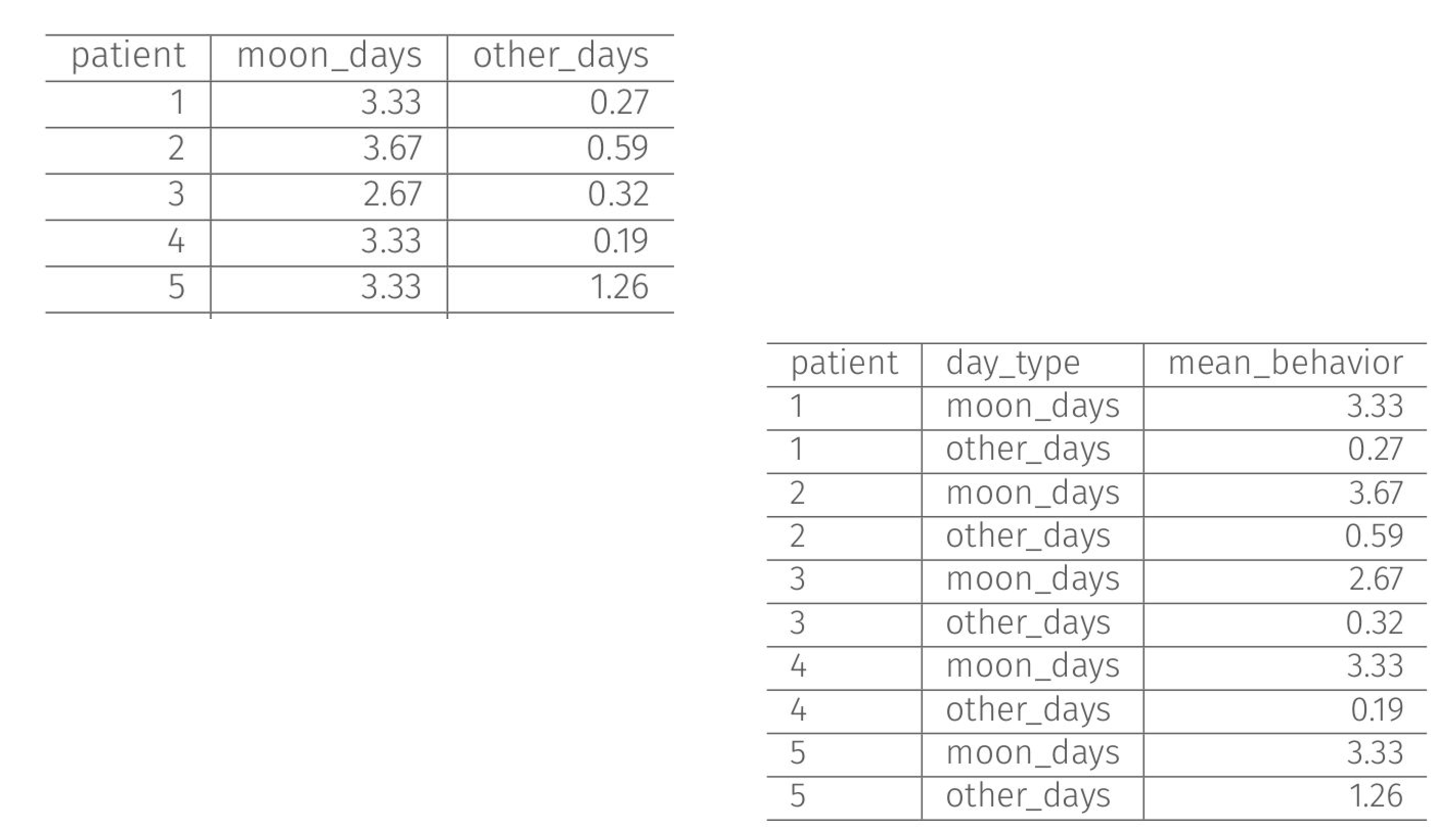
\includegraphics[scale=0.45]{001-tidy3.pdf}
	
	
	%\framedgraphiccaption{tidy-fullmoon.jpg}{\texttt{text}}
	%}
	
\end{frame}

\begin{frame}[fragile]{Not tidy vs. tidy data}
	
	
	%\Wider[4em]{
	%\centering
	
	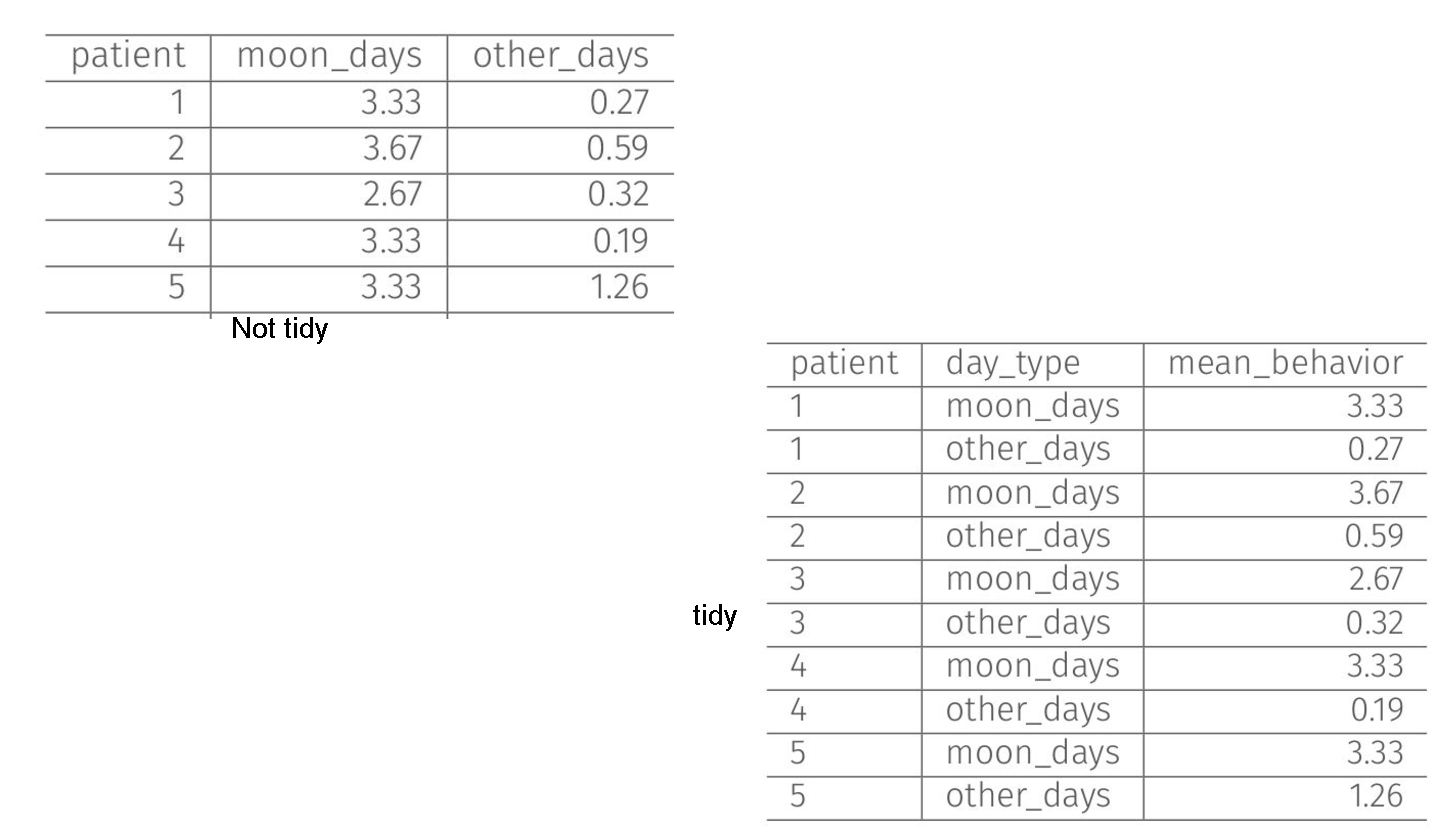
\includegraphics[scale=0.45]{001-tidy4.pdf}
	
	
	%\framedgraphiccaption{tidy-fullmoon.jpg}{\texttt{text}}
	%}
	
\end{frame}







\begin{frame}[fragile]{\texttt{tidyr::pivot\_longer()}}
	
	
	%\Wider[4em]{
	%\centering
	
	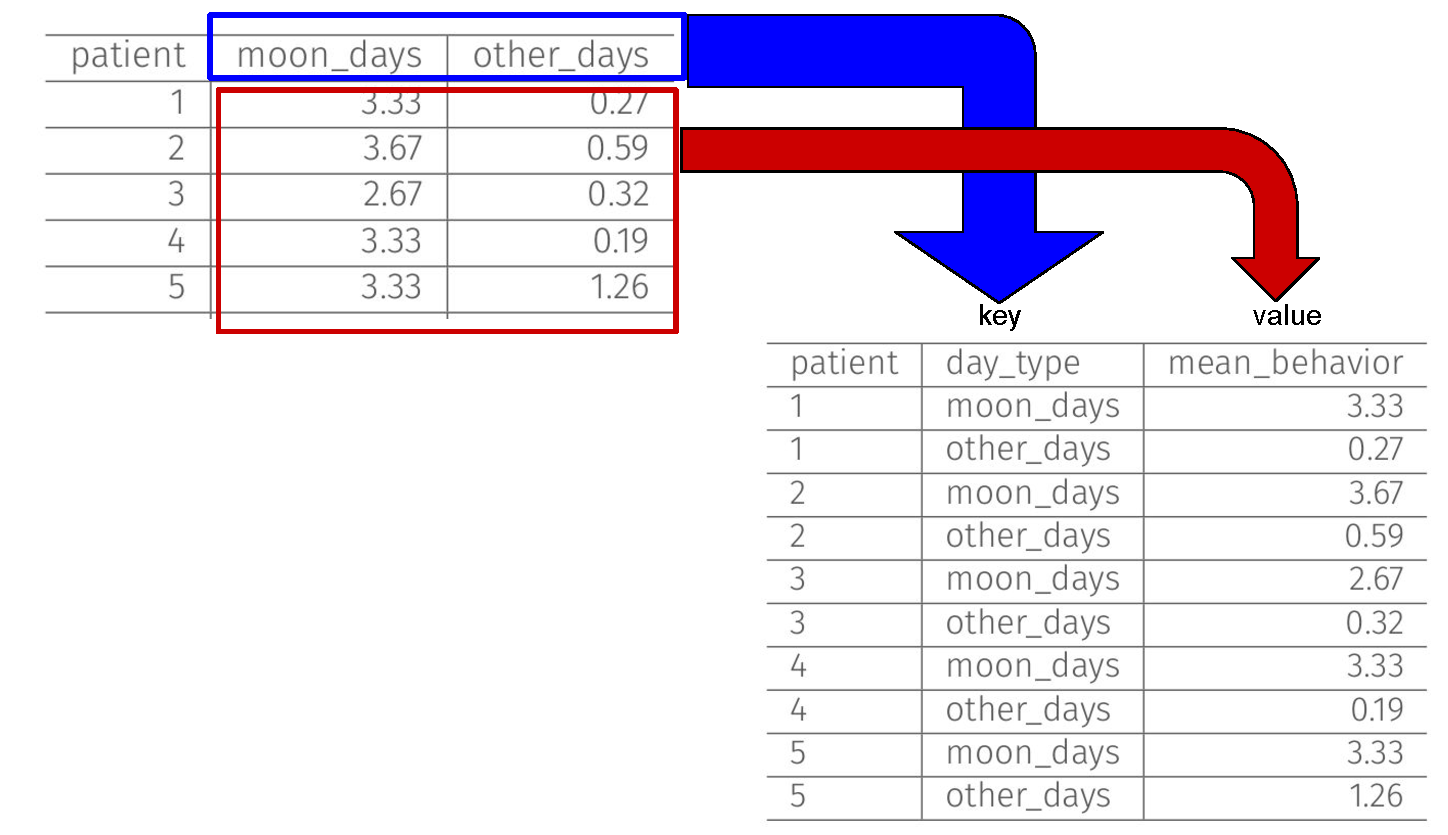
\includegraphics[scale=0.45]{001-tidy1.pdf}
	
	%\pause
	
\begin{knitrout}\tiny
\definecolor{shadecolor}{rgb}{0.969, 0.969, 0.969}\color{fgcolor}\begin{kframe}
\begin{alltt}
\hlstd{tidyr}\hlopt{::}\hlkwd{pivot_longer}\hlstd{(}\hlkwc{data} \hlstd{= df,} \hlkwc{cols} \hlstd{=} \hlopt{-}\hlstd{patient,} \hlkwc{names_to} \hlstd{=} \hlstr{"day_type"}\hlstd{,} \hlkwc{values_to} \hlstd{=} \hlstr{"mean_behavior"}\hlstd{)}
\end{alltt}
\end{kframe}
\end{knitrout}
	
	%\framedgraphiccaption{tidy-fullmoon.jpg}{\texttt{text}}
	%}
	
\end{frame}



\section{Learn regression}


\begin{frame}{Traditional stats textbook}
	\Wider[4em]{
	\centering
	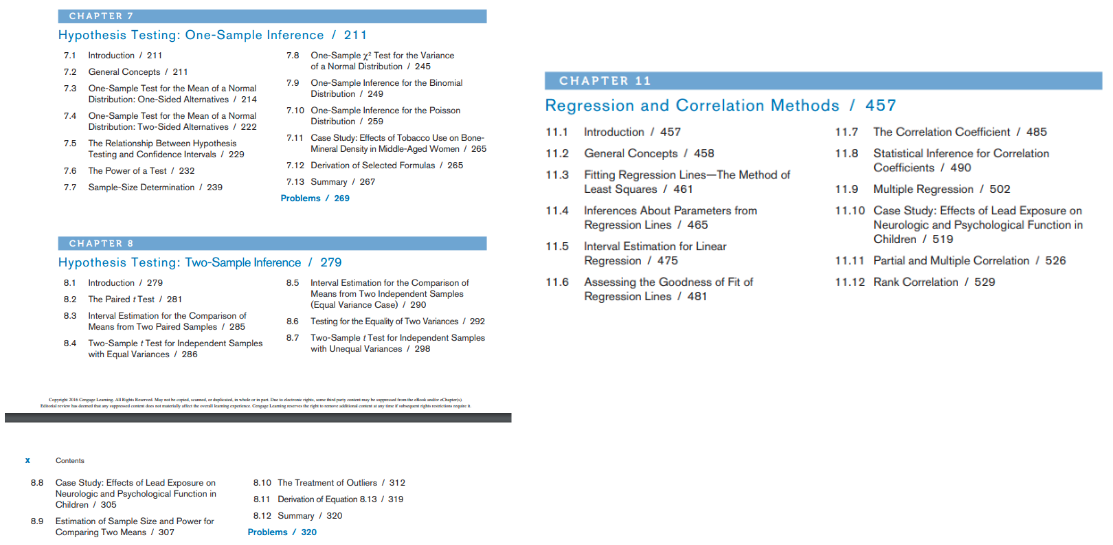
\includegraphics[scale=0.4]{001-text1.png}
}
\end{frame}

\begin{frame}[plain]
	\hspace*{-1.0cm}\parbox[t]{\textwidth}{
		\begin{tikzpicture}[node distance=1.4cm]
		\tikzstyle{every node}=[font=\scriptsize]
		
		% 1st level
		\node (start) [startstopstats] {Parameter};
		
		
		% 2nd level
		\node (mean) [iostats, below of=start, xshift=-3cm] {Mean $\mu$};
		\node (prop) [iostats, below of=start, xshift=3cm] {Proportion $p$};
		
		% 3rd level
		\node (ones) [processbigstats, below of=mean, xshift=-2.5cm] {1 sample $H_0:\mu=\mu_0$};
		\node (match) [processbigstats, below of=mean,xshift=-0.5cm] {Paired \,\,\, $H_0:\mu_1=\mu_2$};
		\node (twos) [processbigstats, below of=mean, xshift=1.5cm] {Unpaired $H_0:\mu_1=\mu_2$};
		
		% 4th level
		\node (onesd) [decisionstats, below of=ones] {$t$ test};
		\node (matchd) [decisionstats, below of=match] {$t$ test on difference};
		\node (twosd) [decisionstats, below of=twos, xshift=-1.0cm, yshift=-1.6cm] {$\sigma_1^2=\sigma_2^2$};
		\node (twosdd) [decisionstats, below of=twos, xshift=1.0cm, yshift=-1.6cm] {$\sigma_1^2\neq\sigma_2^2$};
		
		% 5th level
		\node (onesdtest) [decisionbigstats, below of=onesd, xshift=.7cm,yshift=-1cm] {$t=\frac{\bar{x}-\mu_0}{s/\sqrt{n}} \sim t_{(n-1)} $};
		
		\node (twosdss) [decisionbigstats, below of=twosd,xshift=-.6cm,yshift=-1cm] {$t=\frac{\bar{x}_1-\bar{x}_2}{s_{pooled}\sqrt{ \frac{1}{n_1}+\frac{1}{n_2}  }  } \sim t_{(n_1+n_2-2)}$};
		
		\node (twosdsss) [decisionbigstats, below of=twosdd,yshift=-1cm] {$t=\frac{\bar{x}_1-\bar{x}_2}{\sqrt{ \frac{s_1^2}{n_1}+\frac{s_2^2}{n_2}  }  } \sim t_{min(n_1-1,n_2-1)}$};
		
		% proportions
		
		% 3rd level
		\node (pones) [processbigstats, below of=prop, xshift=-2.2cm] {1 sample $H_0:p=p_0$ };
		\node (ptwos) [processbigstats, below of=prop, xshift=-0.1cm] {2 samples, 2 categories $H_0: p_1=p_2, OR=1, RR=1$};
		\node (ptwoscat) [processbigstats, below of=prop, xshift=2.0cm] {2 samples, multiple categories, $H_0:p_1=p_2$};
		
		% 4th level
		\node (ponesz) [decisionstats, below of=pones] {$z$ test};
		\node (ptwosz) [decisionstats, below of=ptwos, yshift=-1cm] {$z$ or $\chi^2$ test, 95\% CI for OR/RR, Mantel-Haenszel for pooled OR};
		\node (ptwoscatt) [decisionstats, below of=ptwoscat, yshift=-.6cm] {$\chi^2$ test};
		
		
		% 5th level
		\node (ponesztest) [decisionbigstats, below of=ponesz, xshift=1.1cm,yshift=-2.4cm] {$z=\frac{\hat{p}-p_0}{\sqrt{p_0(1-p_0)/n}}, \hat{p}:pooled\,proportion  $};
		\node (ptwosztest) [decisionbigstats, below of=ptwosz, xshift=1.3cm,yshift=-2cm] {$z=\frac{\hat{p}_1-\hat{p}_2}{\sqrt{\hat{p}(1-\hat{p})\left(\frac{1}{n_1}+\frac{1}{n_2}\right)}  }$};
		\node (ptwoscattest) [decisionbigstats, below of=ptwoscatt, yshift=-.8cm] {$\chi^2=\sum\frac{(O-E)^2}{E} \sim \chi^2_{(2-1)(c-1)}  $};
		
		\draw [arrow] (start) -- (mean);
		\draw [arrow] (start) -- (prop);
		\draw [arrow] (mean) -- (ones);
		\draw [arrow] (mean) -- (match);
		\draw [arrow] (mean) -- (twos);
		\draw [arrow] (ones) -- (onesd);
		\draw [arrow] (match) -- (matchd);
		\draw [arrow] (twos) -- (twosd);
		\draw [arrow] (twos) -- (twosdd);
		
		\draw [arrow] (onesd) -- (onesdtest);
		\draw [arrow] (matchd) -- (onesdtest);
		
		\draw [arrow] (twosd) -- (twosdss);
		\draw [arrow] (twosdd) -- (twosdsss);
		
		
		\draw [arrow] (pones) -- (ponesz);
		\draw [arrow] (ptwos) -- (ptwosz);
		\draw [arrow] (ptwoscat) -- (ptwoscatt);
		
		
		\draw [arrow] (ponesz) -- (ponesztest);
		\draw [arrow] (ptwosz) -- (ptwosztest);
		\draw [arrow] (ptwoscatt) -- (ptwoscattest);
		
		
		\draw [arrow] (prop) -- (pones);
		\draw [arrow] (prop) -- (ptwos);
		\draw [arrow] (prop) -- (ptwoscat);
		
		
		
		%%%%%%%%%%%%
		
		\end{tikzpicture}
		
	}
\end{frame}


\begin{frame}{This course}
		\Wider[4em]{
	\centering
	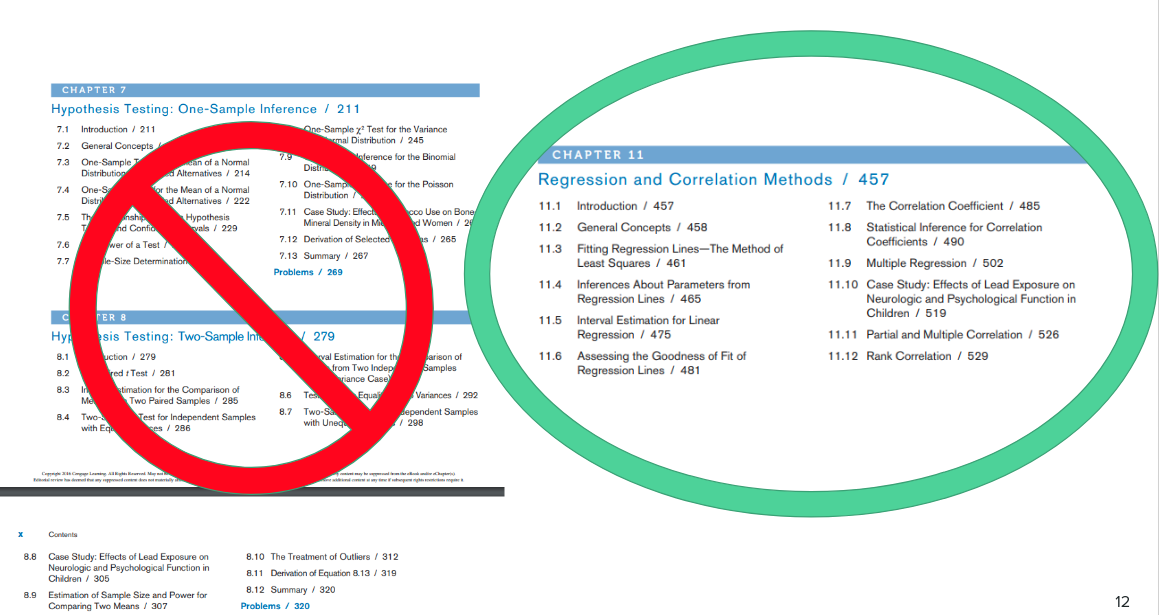
\includegraphics[scale=0.4]{001-text2.png}
}
\end{frame}


\section{Understand the statistical results in a scientific paper}

\begin{frame}{Statistical concepts}
			\Wider[4em]{
		\centering
		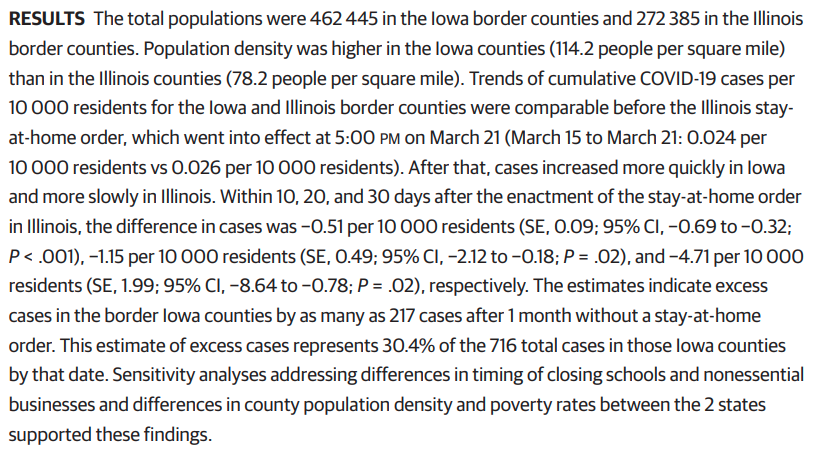
\includegraphics[scale=0.5]{001-jama1.png}
	}
\footnote{\tiny \url{https://jamanetwork.com/journals/jamanetworkopen/fullarticle/2766229}}
\end{frame}


\begin{frame}{Statistical concepts}
	\Wider[4em]{
		\centering
		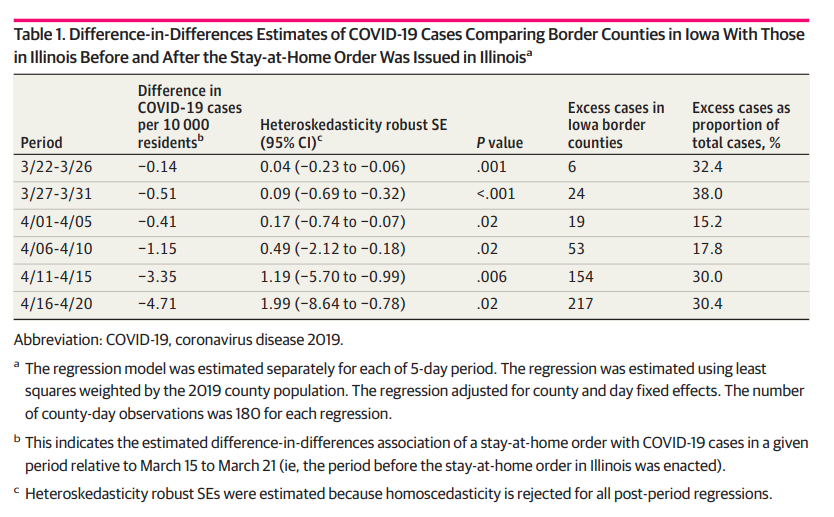
\includegraphics[scale=0.5]{001-jama2.png}
	}
	\footnote{\tiny \url{https://jamanetwork.com/journals/jamanetworkopen/fullarticle/2766229}}
\end{frame}



\section{Learn the tools for creating reproducible analyses}


\begin{frame}{Copy paste ad nauseam}
		\Wider[4em]{
		\centering
		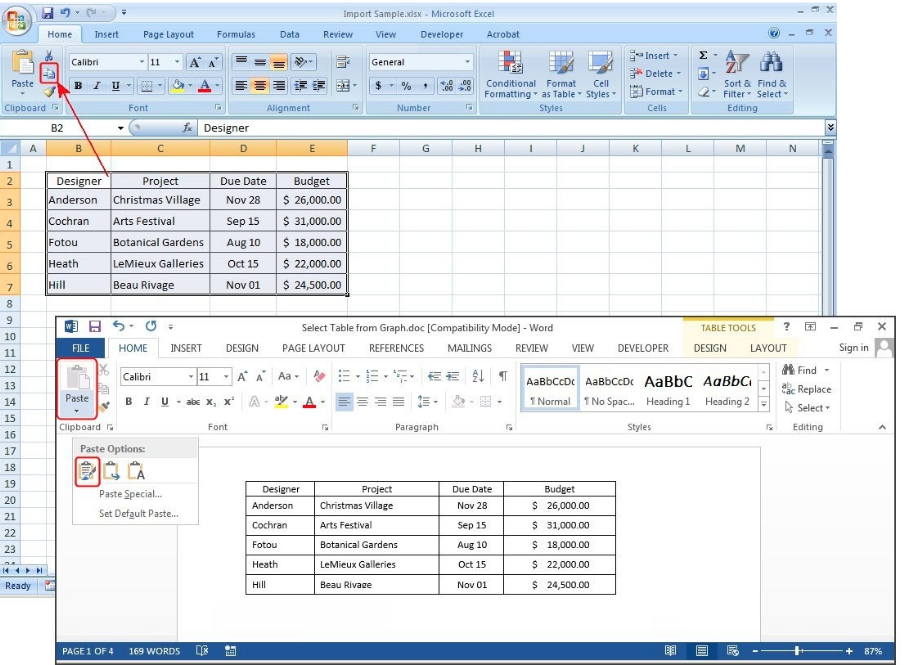
\includegraphics[scale=0.35]{001-excel.png}
	}
\end{frame}


\begin{frame}{Markdown: HTML without knowing HTML}
	\begin{center}
		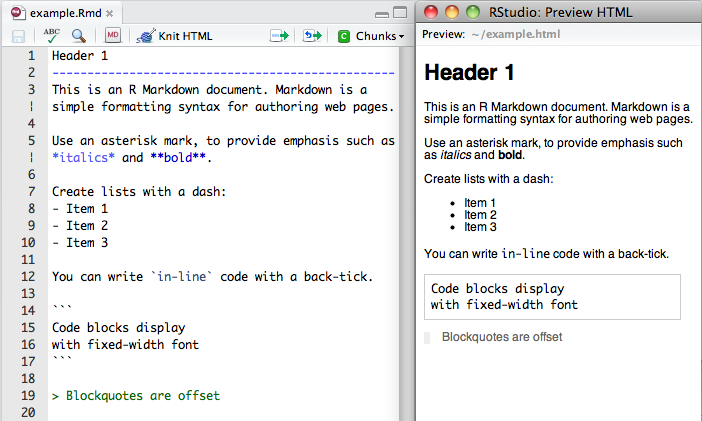
\includegraphics[scale=0.45, keepaspectratio]{001-markdown}
	\end{center}
\end{frame}

\begin{frame}{R + Markdown = RMarkdown}
	\begin{center}
		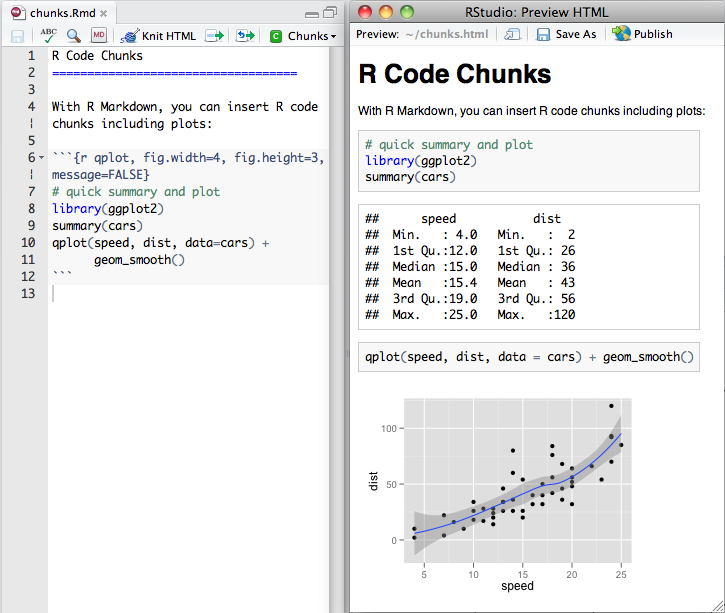
\includegraphics[scale=0.36, keepaspectratio]{001-rmarkdown}
	\end{center}
\end{frame}

\begin{frame}{What \texttt{rmarkdown} does}
	\textbf{\code{RMarkdown}} example:
	
	\begin{center}
		\begin{tikzpicture}
		\scriptsize
		\node (expr) [startstop] {Report.Rmd (contains both code and markdown)};
		\node (science) [decision, below of=expr, xshift=0cm, yshift=-2cm] {Report.md};
		\draw [arrow] (expr) -- node[anchor=east]{\texttt{knitr::knit('Report.Rmd')}} (science);
		\pause \node (pdf) [io, below of=science, xshift=0cm, yshift=-2cm] {Report.html, Report.pdf, Report.doc};
		\draw [arrow] (science) -- node[anchor=east]{\texttt{pandoc}} (pdf);
		\end{tikzpicture}
	\end{center}
\end{frame}


\begin{frame}\frametitle{Compiling a \texttt{.Rmd} document}
	
	\begin{block}{The two steps on previous slide can be executed in one command:}
		\[ \textrm{\texttt{rmarkdown::render()}} \]
	\end{block}
	
	or in \texttt{RStudio}:
	\begin{figure}[h!]
		\centering
		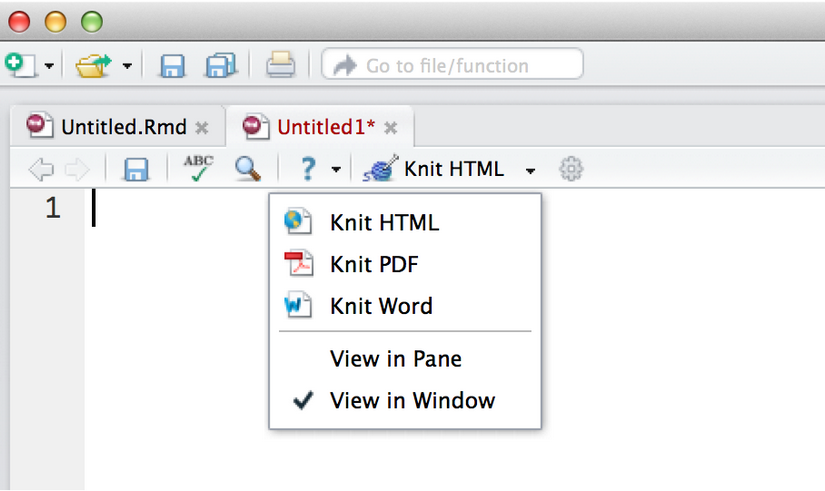
\includegraphics[scale=0.21, keepaspectratio]{001-rmddrop.png}
	\end{figure}
	%\textit{Demonstrate:} Explore \texttt{RStudio}, projects and \texttt{.Rprofile}
\end{frame}


\section{Where does this course fit in my life?}

\begin{frame}{Topics by level of exposure}
			\Wider[4em]{
	\centering
	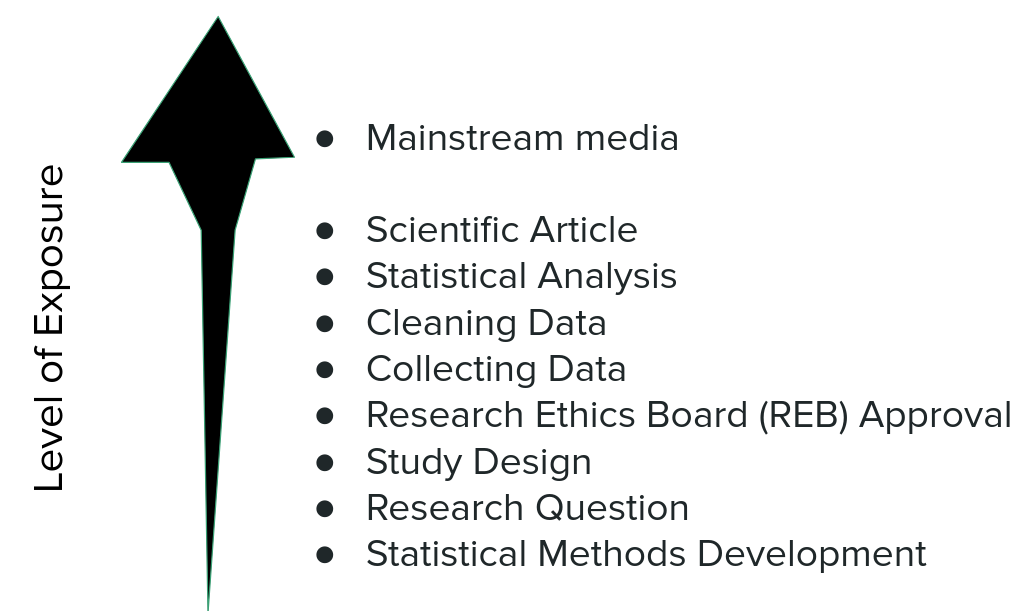
\includegraphics[scale=0.45]{001-persp1.png}
}
\end{frame}

\begin{frame}{First year courses}
	\Wider[4em]{
		\centering
		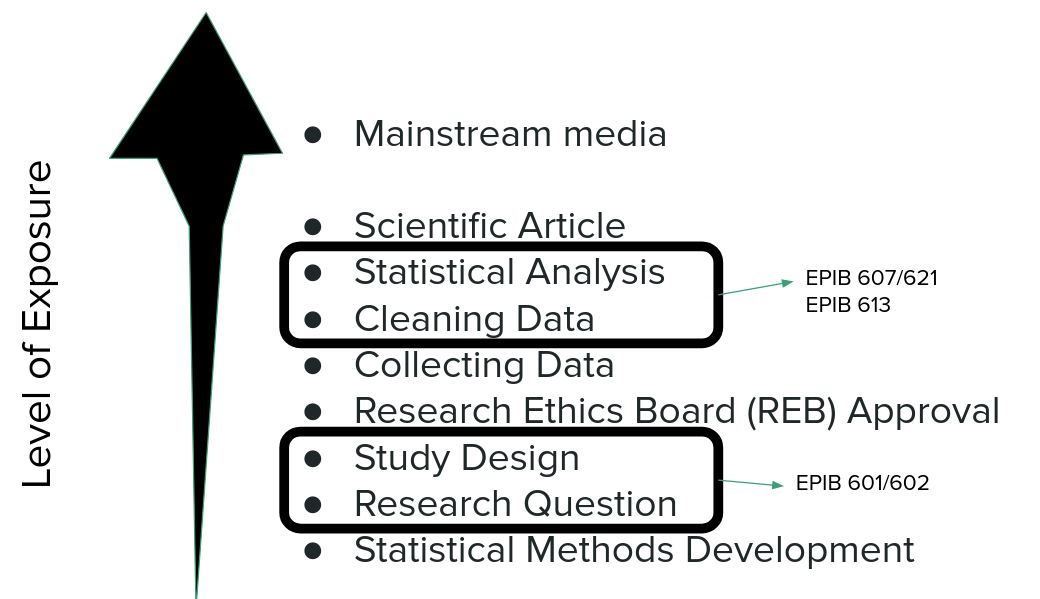
\includegraphics[scale=0.45]{001-persp2.png}
	}
\end{frame}


\begin{frame}{My area of research}
	\Wider[4em]{
		\centering
		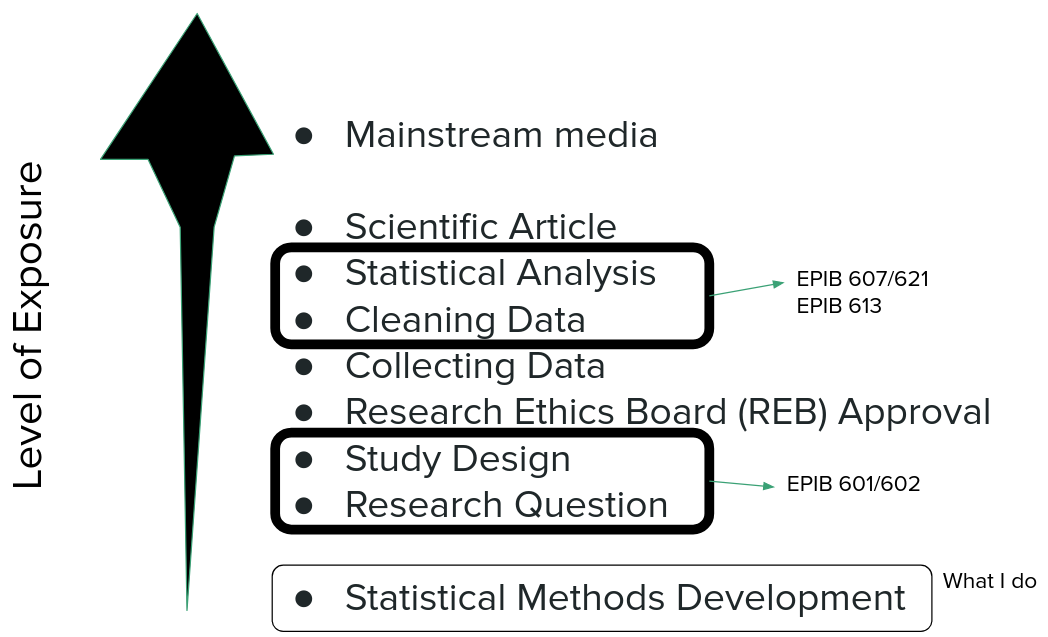
\includegraphics[scale=0.45]{001-persp3.png}
	}
\end{frame}

%\begin{frame}[allowframebreaks]
%\nocite{breiman1984classification}
%	\nocite{friedman2001elements}
%	\nocite{james2013introduction}
%	\nocite{lopez2015arbres}
%	\frametitle{References}
%\printbibliography
%\end{frame}






\begin{frame}[fragile]{Session Info}
	\tiny
	
\begin{knitrout}\tiny
\definecolor{shadecolor}{rgb}{0.969, 0.969, 0.969}\color{fgcolor}\begin{kframe}
\begin{verbatim}
R version 4.0.2 (2020-06-22)
Platform: x86_64-pc-linux-gnu (64-bit)
Running under: Pop!_OS 19.10

Matrix products: default
BLAS:   /usr/lib/x86_64-linux-gnu/openblas-pthread/libblas.so.3
LAPACK: /usr/lib/x86_64-linux-gnu/openblas-pthread/liblapack.so.3

attached base packages:
[1] tools     stats     graphics  grDevices utils     datasets  methods  
[8] base     

other attached packages:
 [1] NCStats_0.4.7   FSA_0.8.30      forcats_0.5.0   stringr_1.4.0  
 [5] dplyr_1.0.2     purrr_0.3.4     readr_1.3.1     tidyr_1.1.2    
 [9] tibble_3.0.3    ggplot2_3.3.2   tidyverse_1.3.0 knitr_1.29     

loaded via a namespace (and not attached):
 [1] nlme_3.1-149       fs_1.5.0           lubridate_1.7.9    httr_1.4.2        
 [5] backports_1.1.9    R6_2.4.1           DBI_1.1.0          colorspace_1.4-1  
 [9] withr_2.2.0        tidyselect_1.1.0   gridExtra_2.3      leaflet_2.0.3     
[13] curl_4.3           compiler_4.0.2     cli_2.0.2          rvest_0.3.6       
[17] xml2_1.3.2         ggdendro_0.1.22    mosaicCore_0.8.0   scales_1.1.1      
[21] digest_0.6.25      minqa_1.2.4        ggformula_0.9.4    foreign_0.8-79    
[25] rio_0.5.16         pkgconfig_2.0.3    htmltools_0.5.0    lme4_1.1-23       
[29] dbplyr_1.4.4       highr_0.8          htmlwidgets_1.5.1  rlang_0.4.7       
[33] readxl_1.3.1       rstudioapi_0.11    farver_2.0.3       generics_0.0.2    
[37] jsonlite_1.7.1     crosstalk_1.1.0.1  zip_2.1.1          car_3.0-9         
[41] magrittr_1.5       mosaicData_0.20.1  Matrix_1.2-18      Rcpp_1.0.5        
[45] munsell_0.5.0      fansi_0.4.1        abind_1.4-5        lifecycle_0.2.0   
[49] stringi_1.5.3      carData_3.0-4      MASS_7.3-53        plyr_1.8.6        
[53] ggstance_0.3.4     grid_4.0.2         blob_1.2.1         ggrepel_0.8.2     
[57] crayon_1.3.4       lattice_0.20-41    haven_2.3.1        splines_4.0.2     
[61] hms_0.5.3          pillar_1.4.6       boot_1.3-25        reprex_0.3.0      
[65] glue_1.4.2         evaluate_0.14      data.table_1.13.0  modelr_0.1.8      
[69] nloptr_1.2.2.2     vctrs_0.3.4        tweenr_1.0.1       cellranger_1.1.0  
[73] gtable_0.3.0       polyclip_1.10-0    assertthat_0.2.1   TeachingDemos_2.12
[77] xfun_0.17          ggforce_0.3.2      openxlsx_4.1.5     broom_0.7.0       
[81] statmod_1.4.34     mosaic_1.7.0       ellipsis_0.3.1    
\end{verbatim}
\end{kframe}
\end{knitrout}

\end{frame}

\end{document}
